\chapter{Funding Ideas: Demonstration Before Capital}

This chapter follows a short School of Hard Knocks exchange, curated by LazyingArt LLC through Video2Book, on the first problem of entrepreneurial funding: what does a founder bring to the table when the company is still mostly an idea? The source segment is an interview rather than a blackboard lecture, so the mathematics here is deliberately modest. We use a small evidence calculus only to make the spoken logic explicit: capital is easier to ask for when the founder can show something real, and advertising polish is weaker than proof that the intended user accepts the product.

\section{The Funding Question}

The opening question is the whole problem in miniature. What should people do when they are trying to get funding for ideas to build companies? We should not rush past that phrasing. The founder begins with an idea, but the investor is being asked to act before the company has fully proven itself.

Let \(I\) denote an idea-only proposal. Let \(D\) denote a demonstrable artifact: a sample, prototype, mockup, or other object that someone can see, test, or react to. Let \(F(X)\) mean the strength of the funding evidence carried by \(X\). This is not a dollar valuation and not a probability; it is a compact way to record the speaker's practical distinction:
\begin{equation}
F(I) < F(I,D).
\end{equation}
The inequality is the first move of the chapter. An idea may be interesting, but a demonstrable thing carries more evidence.

\subsection{Question \& Answer}

\paragraph{Question.}
Can a founder get funding for an idea before the company has anything concrete to show?

\paragraph{Answer.}
The speaker's answer is direct: it always helps to have something demonstrable and not just an idea. Ideas are hard to fund because they leave too much unobserved. A sample or other concrete demonstration changes the conversation. The founder is no longer asking the investor simply to imagine; the founder is offering something that can be inspected.

\section{The Evidence Problem}

An idea has direction, but it has little observed behavior. It may describe a possible customer, a possible product, or a possible market, but it does not yet show that the founder can build, that the product can function, or that the user will care. That is why the speaker says ideas are ``really difficult'' to get funded.

\begin{definition}
For this chapter, an evidence score \(F\) is an ordered measure of how much observable support a founder can show. It is editorial notation, not notation from the interview.
\end{definition}

The idea-only case starts with a weak base:
\begin{equation}
F_0 = F(I).
\end{equation}
The difficulty is not that \(F_0=0\). Some ideas carry evidence through the founder's history, relationships, or reputation. But the ordinary early case in this exchange is different: the idea itself has not yet been made visible.

\begin{remark}
The point of the notation is restraint. We are not inventing a valuation model. We are writing down the local logic of the answer: the investor's uncertainty is high when the founder has only a description.
\end{remark}

\section{The Demonstration Update}

The next beat in the interview is the practical instruction: build something that can be demonstrated. The transcript clearly says ``even just a sample.'' It also contains a likely garbled phrase transcribed as ``especially an attack.'' We should not make that phrase into a term of art. The safe reading is that the speaker means some concrete artifact, however rough, that lets another person see the idea outside the founder's head.

If a demonstration \(D\) is added, the funding evidence updates as
\begin{equation}
F_1 = F(I,D)=F_0+\Delta_D,
\qquad
\Delta_D>0.
\end{equation}
The sign of \(\Delta_D\) carries the lesson. A demonstration does not have to be the finished company. It can be a sample. It can be crude. It can be incomplete. Its value is that it turns part of the claim into something observable.

\paragraph{Worked evidence update.}
The update has a simple structure:
\begin{enumerate}
\item Start with the idea-only proposal \(I\).
\item Assign it an initial evidence level \(F_0=F(I)\).
\item Add a demonstrable artifact \(D\).
\item The evidence becomes \(F_1=F(I,D)\).
\item The speaker's claim is represented by \(F_1-F_0=\Delta_D>0\).
\end{enumerate}
So before asking capital to move, the founder makes the idea visible.

\begin{figure}
\centering
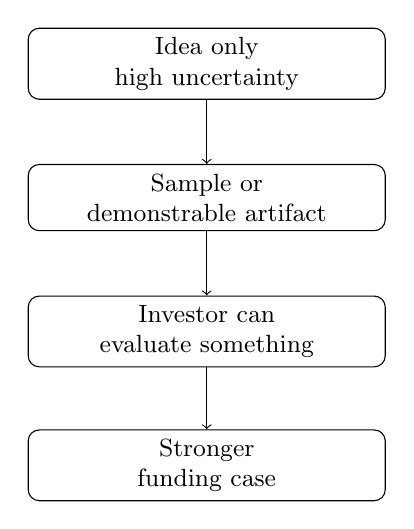
\begin{tikzpicture}[x=1cm,y=1cm,every node/.style={font=\small}]
\node[draw, rounded corners, align=center, text width=4.3cm] (idea) at (0,0) {Idea only\\high uncertainty};
\node[draw, rounded corners, align=center, text width=4.3cm] (demo) at (0,-1.7) {Sample or\\demonstrable artifact};
\node[draw, rounded corners, align=center, text width=4.3cm] (eval) at (0,-3.4) {Investor can\\evaluate something};
\node[draw, rounded corners, align=center, text width=4.3cm] (fund) at (0,-5.1) {Stronger\\funding case};

\draw[->] (idea) -- (demo);
\draw[->] (demo) -- (eval);
\draw[->] (eval) -- (fund);
\end{tikzpicture}
\caption{A transcript-derived evidence ladder: the idea becomes easier to fund when it becomes easier to inspect.}
\end{figure}

\section{The Dog Food Wars Anecdote}

Now the speaker changes mode. Instead of adding more fundraising terminology, he reaches for an old expression, which he places in the 1970s and cautiously associates with the ``dog food wars.'' The claim is anecdotal: advertising companies created many different dog foods, spent money, and put them on television.

The story matters because it tests a tempting shortcut. If funding evidence came merely from presentation, then money spent on promotion should be enough. But that is not the lesson. Let \(A(P)\) denote high advertising exposure for a product \(P\), and let \(U(P)\) denote user acceptance. The bad inference is
\begin{equation}
A(P)\ \hbox{is high}
\quad\Longrightarrow\quad
U(P)\ \hbox{is high}.
\end{equation}
The anecdote is introduced precisely to break that inference:
\begin{equation}
A \uparrow \;\not\Rightarrow\; U \uparrow .
\end{equation}

The product can be visible without being wanted. The campaign can be expensive without validating the product.

\section{The Market Test}

The turn in the story is plain: the dogs did not like the dog food. The intended user rejects the product, and that rejection dominates the advertising story. In the compact notation,
\begin{equation}
A(P)=1,
\qquad
U(P)=0,
\end{equation}
where \(A(P)=1\) means the product has high promotional exposure, while \(U(P)=0\) means the intended user does not accept it.

From the point of view of funding evidence, this is not a strong market signal:
\begin{equation}
A(P)=1,\quad U(P)=0
\quad\Longrightarrow\quad
F(P)\ \hbox{is weak as market proof}.
\end{equation}
That is the conceptual payoff of the anecdote. Advertising can create attention, but it cannot make the user like the product. A demonstration matters because it exposes reality; sometimes reality supports the case, and sometimes it breaks the case.

\begin{figure}
\centering
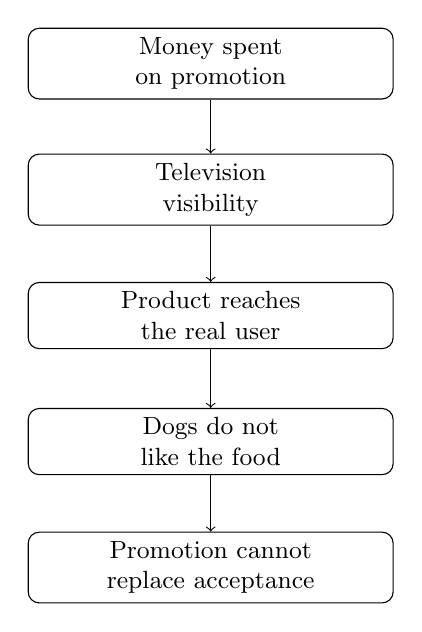
\begin{tikzpicture}[x=1cm,y=1cm,every node/.style={font=\small}]
\node[draw, rounded corners, align=center, text width=4.4cm] (spend) at (0,0) {Money spent\\on promotion};
\node[draw, rounded corners, align=center, text width=4.4cm] (tv) at (0,-1.6) {Television\\visibility};
\node[draw, rounded corners, align=center, text width=4.4cm] (trial) at (0,-3.2) {Product reaches\\the real user};
\node[draw, rounded corners, align=center, text width=4.4cm] (reject) at (0,-4.8) {Dogs do not\\like the food};
\node[draw, rounded corners, align=center, text width=4.4cm] (lesson) at (0,-6.4) {Promotion cannot\\replace acceptance};

\draw[->] (spend) -- (tv);
\draw[->] (tv) -- (trial);
\draw[->] (trial) -- (reject);
\draw[->] (reject) -- (lesson);
\end{tikzpicture}
\caption{The dog-food anecdote as a narrow causal chain: exposure is not validation.}
\end{figure}

\section{Evidence Before Capital}

We can now join the two parts of the exchange. The first part says: if you want funding, bring something demonstrable. The second part says: even expensive presentation is not enough if the product fails the user test. The shared principle is evidence before capital.

A compact way to write the mechanism is
\begin{align}
\hbox{idea only}
&\longrightarrow
\hbox{high investor uncertainty},
\\
\hbox{demonstrable artifact}
&\longrightarrow
\hbox{lower investor uncertainty},
\\
\hbox{real user acceptance}
&\longrightarrow
\hbox{stronger market proof}.
\end{align}
The negative version is just as important:
\begin{equation}
\hbox{flashy presentation} \not\equiv \hbox{validated demand}.
\end{equation}

So the founder's first job is not simply to persuade harder. It is to make the claim more testable. A sample, a prototype, or a visible product trial converts part of the story into evidence. Once the idea has a surface that other people can touch, inspect, or reject, the funding conversation becomes more serious.

\section{Summary}

The lecture's rhythm is short but complete. It begins with a founder's funding question, answers with the need for something demonstrable, and then uses the dog-food anecdote to separate promotion from validation. The durable rule is not that founders must arrive with a finished company. It is that they should reduce uncertainty before asking others to fund the risk.

In the notation of the chapter, the whole point can be compressed as
\begin{align}
F(I) &< F(I,D),
\\
A \uparrow &\not\Rightarrow U \uparrow,
\\
\hbox{funding strength}
&\sim
\hbox{demonstration}+\hbox{user evidence}.
\end{align}
The careful prose version is even simpler: before asking investors to believe, give them something real to evaluate.